\documentclass[justified,nobib]{tufte-handout}
\usepackage{microtype}
\usepackage[english]{babel}
\usepackage{inputenc}
\usepackage{graphicx}
\usepackage{amsthm}
\usepackage{amsmath}
\usepackage{amssymb}
\usepackage{listings}
\usepackage{hyperref}
\usepackage{bm}
\lstdefinestyle{mystyle}{
    % backgroundcolor=\color{backcolour},   
    commentstyle=\color{magenta},
    % keywordstyle=\color{magenta},
    numberstyle=\tiny\color{gray},
    % stringstyle=\color{codepurple},
    basicstyle=\ttfamily\small,
    breakatwhitespace=false,         
    breaklines=true,                 
    captionpos=b,                    
    keepspaces=true,                 
    numbers=left,                    
    numbersep=5pt,                  
    showspaces=false,                
    showstringspaces=false,
    showtabs=false,                  
    tabsize=2
}
\lstset{style=mystyle}


\usepackage[square,sort,comma,numbers]{natbib}
\title{ece467 - Final Project}
\author{Armaan Kohli}
\date{\today}
\begin{document}
\begin{fullwidth}
\selectlanguage{English}
{
  \noindent\fontsize{12pt}{20pt}\selectfont\textbf{Final Project: Character-Level Language Modeling for Text Generation via Deep Markov Models}
  \newline
  \fontsize{12pt}{18pt}\selectfont
  {Armaan Kohli - \scshape ece}467 Natural Language Processing \\Spring 2020\\
}
\raggedright
\raggedbottom
\section{Remarks}
\paragraph{} We attempted to use a deep markov model (DMM) to make a character-level language model. This work is based on recent developments in the understanding of discrete time series, such as MIDI, as well as natural language processing. Using a DMM, we were able to generate text that yielded quantitative performance approaching state of the art for character-based language models. However, training remains unstable and more research into DMMs is likely required for their performance for language models to improve. 

\section{Deep Markov Models}
\paragraph{}
Traditional markov models are a method representing complex temporal dependencies in observed data. A markov model has a chain of latent variables, with each latent (or hidden) variable in the chain is conditioned on the previous latent variable. This is a useful approach, but if we want to represent complex data with complex dynamics, such as text, we would like to be able to model dynamics that are potentially highly non-linear.
\end{fullwidth}
\begin{marginfigure}[1.5in]
\includegraphics[scale=.35]{./media/pyro.png}
\caption{An illustration of a DMM. Each of the black squares represent an RNNs that determine the probability of emission or transmission. Image replicated from Pyro documentation \cite{pyro}}
\label{fig:dmm}
\end{marginfigure}
\paragraph{} This brings forth the idea of a deep markov model, wherein we allow the transition probabilities governing the dynamics of the latent variables as well as the the emission probabilities that govern how the observations are generated by the latent dynamics to be parametrized by (non-linear) neural networks.
DMMs were first used in the setting of polyphonic music generation. Using a MIDI representation of musical notes, Krishnan et. al were able to generate high-quality songs and learn a representaton of electronic health record data \cite{dmm}. 

\paragraph{} Even though this method was originally designed for music generation, character-level language models can be thought of in a similar \begin{fullwidth}
way. At each time step, music can be represented by an 88-dimensional binary vector. Similarly, characters in a phrase can be represented by a one-hot vector with a dimension given by the size of the learned dictionary. Research by the Harvard Intellegnt Probabalistic Systems (HIPS) group takes a similar approach, using the a neural network for both polyphonic music generation and character-level language modeling, the only change being the distribution from which the data is drawn from, the obervation liklihod (Bernoulli vs categorical) \cite{discreteflow}. HIPS uses a generative flow model for character-level language modelling as opposed to a DMM, however. The inference strategy we're going to use called variational inference (VI), which requires specifying a parametrized family of distributions that can be used to approximate the posterior distribution over the latent random variables. Due to the complex temporal relations we seek to model, we can expect the posterior distribution to be highly non-trivial, necessitating a probabilistic approach. Thus, we use \texttt{PyTorch} as our choice of deep learning framework, as well as \texttt{Pyro}, a probabilistic programming language integrated into \texttt{PyTorch} to effectively sample and perform VI on our model.
 
\section{Implementation Details} 
\paragraph{}
 We use a single-layer RNN for our emission and transmission probabilities. Our objective function is the ELBO (evidence-based lower bound) with a KL-annealing term $\beta$, inspired by \cite{bvae}.
 \begin{equation}
\mathcal{F}(\theta,\phi,\beta;\bm{x},\bm{z}) \geq \mathcal{L}(\theta,\phi;\bm{x},\bm{z}) = \mathbb{E}_{q_{\phi}(z|x)}[log_{p_{\theta}}(\bm{x}|\bm{z})]-\beta D_{KL}(q_{\phi}(\bm{z}|\bm{x})||p(\bm{z}))
\end{equation} 
We use Monte Carlo estimates of the KL divergence term. 
\paragraph{} We train the language model using the Penn Treebank (PTB) corpus. We perform treat every line in the corpus as a distinct sequence, or sentence, and tokenize each character in each sentence, adding the \texttt{<unk>} token for low-frequency or unknown words, and \texttt{<eos>} to demarcate the end of a sentence. The size of the dictionary was 52. In order to generate a character embedding, we simply encoded our character dictionary as a one-hot 52-dimensional vector. This was an appropriate choice due to the small dictionary size. We opt for a batch size of 16. For full details see \underline{\href{https://github.com/armaank/textDMM}{github.com/armaank/textDMM}} for the full codebase and the parameters used to train the network.
\paragraph{} We found that using the entirety of the PTB dataset to be challenging for our language model. The longer the sentence used in the character level language model, the more difficult the model was to optimize. We found that limiting ourselves to sentences shorter than 50 characters significantly improved results. However, this would mean that the semantic quality of generated sentences would be reduced as the length of the sentence increases. 

\section{Results \& Discussion}

\paragraph{} Figure \ref{fig:loss} illustrates the negative log likelihood learning curve, showing that the model converges. 
\begin{figure}[h]
\caption{}
\centering
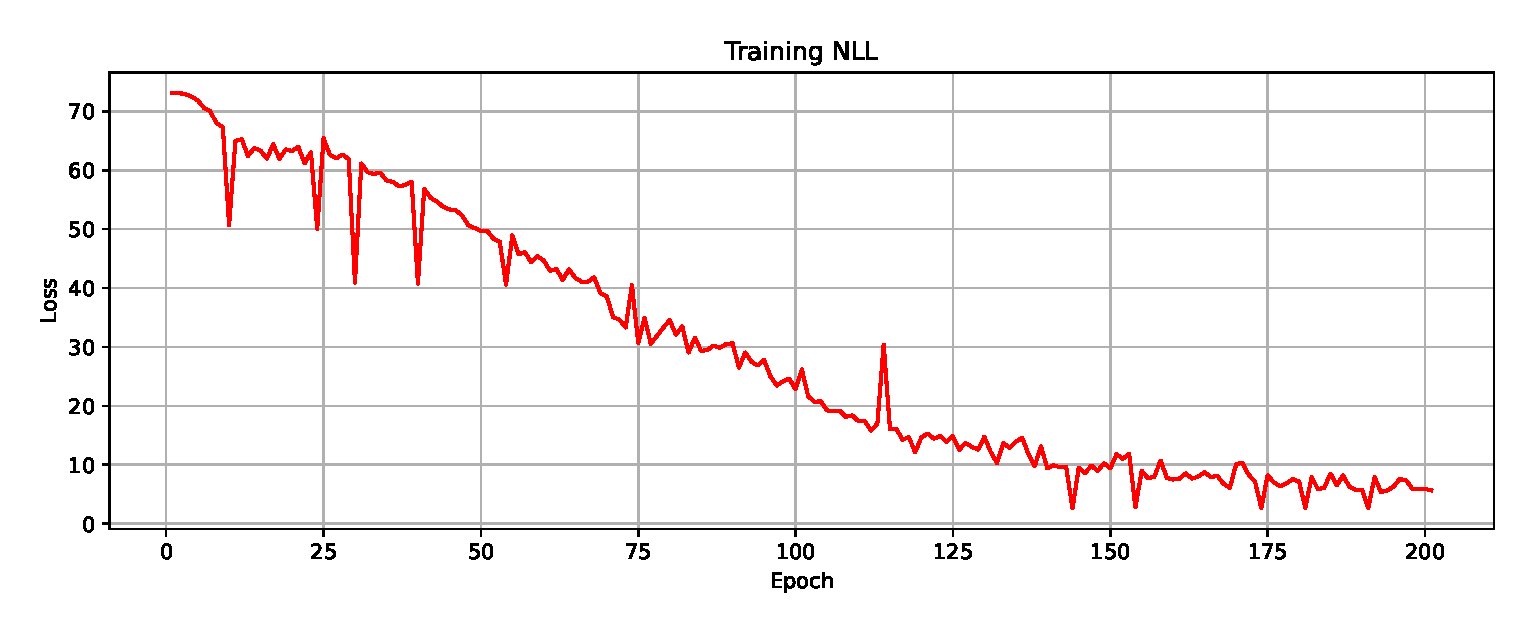
\includegraphics[width=\textwidth]{./media/loss.eps}
\label{fig:loss}
\end{figure}\\
In order to see if our implementation is reasonable we compared our results to the numbers reported in \cite{discreteflow} in Table \ref{tab:results}\\
\begin{center} 
\begin{table}[htp]
\label{tab:results}
\begin{tabular}{ll}
\hline
\multicolumn{2}{c}{NLL Validation/Test Loss} \\ \hline
\multicolumn{1}{l|}{LSTM} & 1.38  \\ \hline
\multicolumn{1}{l|}{AWD-LSTM} & 1.18  \\ \hline
\multicolumn{1}{l|}{IAF} & 1.42  \\ \hline
\multicolumn{1}{l|}{DMM} & 6.82 \\ \hline
\end{tabular}
\caption{This table compares the various results of state of the art character level language models. The results for the LSTM, AWD-LSTM and IAF come from \cite{discreteflow}}
\end{table}
\end{center}
\paragraph{} The LSTM, AWD-LSTM and IAF are state of the art language models. These langauge models were able to train for much longer durations and were able to use a larger portion of the PTB dataset because they could use long sentences. Our results are fairly close to the others in terms of NLL loss, which appears to be the standard performance metric in character-level language modelling tasks.

\paragraph{} Performance of the DMM might be improve by using a different method for KL annealing, which can improve stability during training. Furthermore, we use a Monte Carlo estimate of the KL divergence, leading to higher variance gradient estimates of the ELBO loss, which can also destabilize performance during early training periods. We might also trying using an LSTM architecture to parametrize our transmission and emission probabilities over the so-called `vanilla' RNN. On a related note, one possibility is that exploding gradients are caused by lengthy input sequences, so one way to resolve this issue would be to only train on shorter sequences of characters. 

\section{Conclusion}

\paragraph{} In conclusion, we were able to successfully train a DMM as a character-level language model and achieve strong performance. However, though more research is needed to improve DMMs for NLP tasks.

\bibliography{bib}{}
\bibliographystyle{IEEEtran}
\clearpage
\section{Appendix A: Code}
The code below is \texttt{dmm.py}, the main model code. 
\lstinputlisting[language=Python,frame=single]{../../dmm.py}
\clearpage
The code below is \texttt{train.py}, the main code used to perform training and evaluation.
\lstinputlisting[language=Python,frame=single]{../../train.py}
\end{fullwidth}

\end{document}